% Options for packages loaded elsewhere
\PassOptionsToPackage{unicode}{hyperref}
\PassOptionsToPackage{hyphens}{url}
%
\documentclass[
]{book}
\usepackage{lmodern}
\usepackage{amsmath}
\usepackage{ifxetex,ifluatex}
\ifnum 0\ifxetex 1\fi\ifluatex 1\fi=0 % if pdftex
  \usepackage[T1]{fontenc}
  \usepackage[utf8]{inputenc}
  \usepackage{textcomp} % provide euro and other symbols
  \usepackage{amssymb}
\else % if luatex or xetex
  \usepackage{unicode-math}
  \defaultfontfeatures{Scale=MatchLowercase}
  \defaultfontfeatures[\rmfamily]{Ligatures=TeX,Scale=1}
\fi
% Use upquote if available, for straight quotes in verbatim environments
\IfFileExists{upquote.sty}{\usepackage{upquote}}{}
\IfFileExists{microtype.sty}{% use microtype if available
  \usepackage[]{microtype}
  \UseMicrotypeSet[protrusion]{basicmath} % disable protrusion for tt fonts
}{}
\makeatletter
\@ifundefined{KOMAClassName}{% if non-KOMA class
  \IfFileExists{parskip.sty}{%
    \usepackage{parskip}
  }{% else
    \setlength{\parindent}{0pt}
    \setlength{\parskip}{6pt plus 2pt minus 1pt}}
}{% if KOMA class
  \KOMAoptions{parskip=half}}
\makeatother
\usepackage{xcolor}
\IfFileExists{xurl.sty}{\usepackage{xurl}}{} % add URL line breaks if available
\IfFileExists{bookmark.sty}{\usepackage{bookmark}}{\usepackage{hyperref}}
\hypersetup{
  pdftitle={의학연구에서의 실험계획법 소개},
  pdfauthor={서울시립대 통계학과},
  hidelinks,
  pdfcreator={LaTeX via pandoc}}
\urlstyle{same} % disable monospaced font for URLs
\usepackage{color}
\usepackage{fancyvrb}
\newcommand{\VerbBar}{|}
\newcommand{\VERB}{\Verb[commandchars=\\\{\}]}
\DefineVerbatimEnvironment{Highlighting}{Verbatim}{commandchars=\\\{\}}
% Add ',fontsize=\small' for more characters per line
\usepackage{framed}
\definecolor{shadecolor}{RGB}{248,248,248}
\newenvironment{Shaded}{\begin{snugshade}}{\end{snugshade}}
\newcommand{\AlertTok}[1]{\textcolor[rgb]{0.94,0.16,0.16}{#1}}
\newcommand{\AnnotationTok}[1]{\textcolor[rgb]{0.56,0.35,0.01}{\textbf{\textit{#1}}}}
\newcommand{\AttributeTok}[1]{\textcolor[rgb]{0.77,0.63,0.00}{#1}}
\newcommand{\BaseNTok}[1]{\textcolor[rgb]{0.00,0.00,0.81}{#1}}
\newcommand{\BuiltInTok}[1]{#1}
\newcommand{\CharTok}[1]{\textcolor[rgb]{0.31,0.60,0.02}{#1}}
\newcommand{\CommentTok}[1]{\textcolor[rgb]{0.56,0.35,0.01}{\textit{#1}}}
\newcommand{\CommentVarTok}[1]{\textcolor[rgb]{0.56,0.35,0.01}{\textbf{\textit{#1}}}}
\newcommand{\ConstantTok}[1]{\textcolor[rgb]{0.00,0.00,0.00}{#1}}
\newcommand{\ControlFlowTok}[1]{\textcolor[rgb]{0.13,0.29,0.53}{\textbf{#1}}}
\newcommand{\DataTypeTok}[1]{\textcolor[rgb]{0.13,0.29,0.53}{#1}}
\newcommand{\DecValTok}[1]{\textcolor[rgb]{0.00,0.00,0.81}{#1}}
\newcommand{\DocumentationTok}[1]{\textcolor[rgb]{0.56,0.35,0.01}{\textbf{\textit{#1}}}}
\newcommand{\ErrorTok}[1]{\textcolor[rgb]{0.64,0.00,0.00}{\textbf{#1}}}
\newcommand{\ExtensionTok}[1]{#1}
\newcommand{\FloatTok}[1]{\textcolor[rgb]{0.00,0.00,0.81}{#1}}
\newcommand{\FunctionTok}[1]{\textcolor[rgb]{0.00,0.00,0.00}{#1}}
\newcommand{\ImportTok}[1]{#1}
\newcommand{\InformationTok}[1]{\textcolor[rgb]{0.56,0.35,0.01}{\textbf{\textit{#1}}}}
\newcommand{\KeywordTok}[1]{\textcolor[rgb]{0.13,0.29,0.53}{\textbf{#1}}}
\newcommand{\NormalTok}[1]{#1}
\newcommand{\OperatorTok}[1]{\textcolor[rgb]{0.81,0.36,0.00}{\textbf{#1}}}
\newcommand{\OtherTok}[1]{\textcolor[rgb]{0.56,0.35,0.01}{#1}}
\newcommand{\PreprocessorTok}[1]{\textcolor[rgb]{0.56,0.35,0.01}{\textit{#1}}}
\newcommand{\RegionMarkerTok}[1]{#1}
\newcommand{\SpecialCharTok}[1]{\textcolor[rgb]{0.00,0.00,0.00}{#1}}
\newcommand{\SpecialStringTok}[1]{\textcolor[rgb]{0.31,0.60,0.02}{#1}}
\newcommand{\StringTok}[1]{\textcolor[rgb]{0.31,0.60,0.02}{#1}}
\newcommand{\VariableTok}[1]{\textcolor[rgb]{0.00,0.00,0.00}{#1}}
\newcommand{\VerbatimStringTok}[1]{\textcolor[rgb]{0.31,0.60,0.02}{#1}}
\newcommand{\WarningTok}[1]{\textcolor[rgb]{0.56,0.35,0.01}{\textbf{\textit{#1}}}}
\usepackage{longtable,booktabs}
\usepackage{calc} % for calculating minipage widths
% Correct order of tables after \paragraph or \subparagraph
\usepackage{etoolbox}
\makeatletter
\patchcmd\longtable{\par}{\if@noskipsec\mbox{}\fi\par}{}{}
\makeatother
% Allow footnotes in longtable head/foot
\IfFileExists{footnotehyper.sty}{\usepackage{footnotehyper}}{\usepackage{footnote}}
\makesavenoteenv{longtable}
\usepackage{graphicx}
\makeatletter
\def\maxwidth{\ifdim\Gin@nat@width>\linewidth\linewidth\else\Gin@nat@width\fi}
\def\maxheight{\ifdim\Gin@nat@height>\textheight\textheight\else\Gin@nat@height\fi}
\makeatother
% Scale images if necessary, so that they will not overflow the page
% margins by default, and it is still possible to overwrite the defaults
% using explicit options in \includegraphics[width, height, ...]{}
\setkeys{Gin}{width=\maxwidth,height=\maxheight,keepaspectratio}
% Set default figure placement to htbp
\makeatletter
\def\fps@figure{htbp}
\makeatother
\setlength{\emergencystretch}{3em} % prevent overfull lines
\providecommand{\tightlist}{%
  \setlength{\itemsep}{0pt}\setlength{\parskip}{0pt}}
\setcounter{secnumdepth}{5}
%----- my options----------------
\usepackage[hangul]{kotex}
\usepackage{bm}
\usepackage{fullpage}

\newcommand{\pardiff}[2]{\frac{\partial #1}{\partial #2 }}
\newcommand{\pardiffl}[2]{{\partial #1}/{\partial #2 }}
\newcommand{\pardiffd}[2]{\frac{\partial^2 #1}{\partial #2^t \partial #2 }}
\newcommand{\pardiffdd}[3]{\frac{\partial^2 #1}{\partial #2 \partial #3 }}


%--------- from bookdown.org --------------

\usepackage{booktabs}


\usepackage{framed,color}
\definecolor{shadecolor}{RGB}{248,248,248}

\renewcommand{\textfraction}{0.05}
\renewcommand{\topfraction}{0.8}
\renewcommand{\bottomfraction}{0.8}
\renewcommand{\floatpagefraction}{0.75}

\renewenvironment{quote}{\begin{VF}}{\end{VF}}
\let\oldhref\href
\renewcommand{\href}[2]{#2\footnote{\url{#1}}}

\makeatletter
\newenvironment{kframe}{%
\medskip{}
\setlength{\fboxsep}{.8em}
 \def\at@end@of@kframe{}%
 \ifinner\ifhmode%
  \def\at@end@of@kframe{\end{minipage}}%
  \begin{minipage}{\columnwidth}%
 \fi\fi%
 \def\FrameCommand##1{\hskip\@totalleftmargin \hskip-\fboxsep
 \colorbox{shadecolor}{##1}\hskip-\fboxsep
     % There is no \\@totalrightmargin, so:
     \hskip-\linewidth \hskip-\@totalleftmargin \hskip\columnwidth}%
 \MakeFramed {\advance\hsize-\width
   \@totalleftmargin\z@ \linewidth\hsize
   \@setminipage}}%
 {\par\unskip\endMakeFramed%
 \at@end@of@kframe}
\makeatother

\makeatletter

\@ifundefined{Shaded}{
}{\renewenvironment{Shaded}{\begin{kframe}}{\end{kframe}}}
\makeatother

\newenvironment{rmdblock}[1]
  {
  \begin{itemize}
  \renewcommand{\labelitemi}{
    \raisebox{-.7\height}[0pt][0pt]{
      {\setkeys{Gin}{width=3em,keepaspectratio}\includegraphics{images/#1}}
    }
  }
  \setlength{\fboxsep}{1em}
  \begin{kframe}
  \item
  }
  {
  \end{kframe}
  \end{itemize}
  }
  
\newenvironment{rmdnote}
  {\begin{rmdblock}{note}}
  {\end{rmdblock}}
  
\newenvironment{rmdcaution}
  {\begin{rmdblock}{caution}}
  {\end{rmdblock}}
  
\newenvironment{rmdimportant}
  {\begin{rmdblock}{important}}
  {\end{rmdblock}}
  
\newenvironment{rmdtip}
  {\begin{rmdblock}{tip}}
  {\end{rmdblock}}
  
\newenvironment{rmdwarning}
  {\begin{rmdblock}{warning}}
  {\end{rmdblock}}
  


\usepackage{makeidx}
\makeindex

\urlstyle{tt}

\usepackage{amsthm}
\makeatletter
 \def\thm@space@setup{%
   \thm@preskip=8pt plus 2pt minus 4pt
   \thm@postskip=\thm@preskip
}
\makeatother

\frontmatter
\usepackage{booktabs}
\usepackage{longtable}
\usepackage{array}
\usepackage{multirow}
\usepackage{wrapfig}
\usepackage{float}
\usepackage{colortbl}
\usepackage{pdflscape}
\usepackage{tabu}
\usepackage{threeparttable}
\usepackage{threeparttablex}
\usepackage[normalem]{ulem}
\usepackage{makecell}
\usepackage{xcolor}
\ifluatex
  \usepackage{selnolig}  % disable illegal ligatures
\fi
\usepackage[]{natbib}
\bibliographystyle{apalike}

\title{의학연구에서의 실험계획법 소개}
\author{서울시립대 통계학과}
\date{2021-05-03}

\begin{document}
\maketitle

{
\setcounter{tocdepth}{1}
\tableofcontents
}
\hypertarget{uxc18cuxac1c}{%
\chapter*{소개}\label{uxc18cuxac1c}}


의학연구에서 임상실험에 나오는 주요 실험 게획법에 대한 소개입니다.

이번 강의에 필요한 \texttt{R}라이브러리는 다음과 같다.

\begin{verbatim}
library(ggplot2)
library(dplyr)
library(tidyr)
library(kableExtra)
library(car)
library(equatiomatic)
\end{verbatim}

\mainmatter

\hypertarget{intro}{%
\chapter{공분산분석}\label{intro}}

의학연구에서는 치료법이나 약물의 효과를 알아보기 위한 다양한 실험이 진행된다.

치료법이나 약품의 효과에 대하여 기초 연구(화학실험, 동물실험 등)가 어느 정도 진행되어 기대되는 효능이 있으며 큰 부작용이 없다고 판단되면 인간에게 치료법을 적용하거나 약품을 사용하는 임상실험(clinical trial)을 진행햔다.

임상실험은 많은 경우 \textbf{병렬 계획(parallel design)}에 의거한 일원배치법을 사용한다.

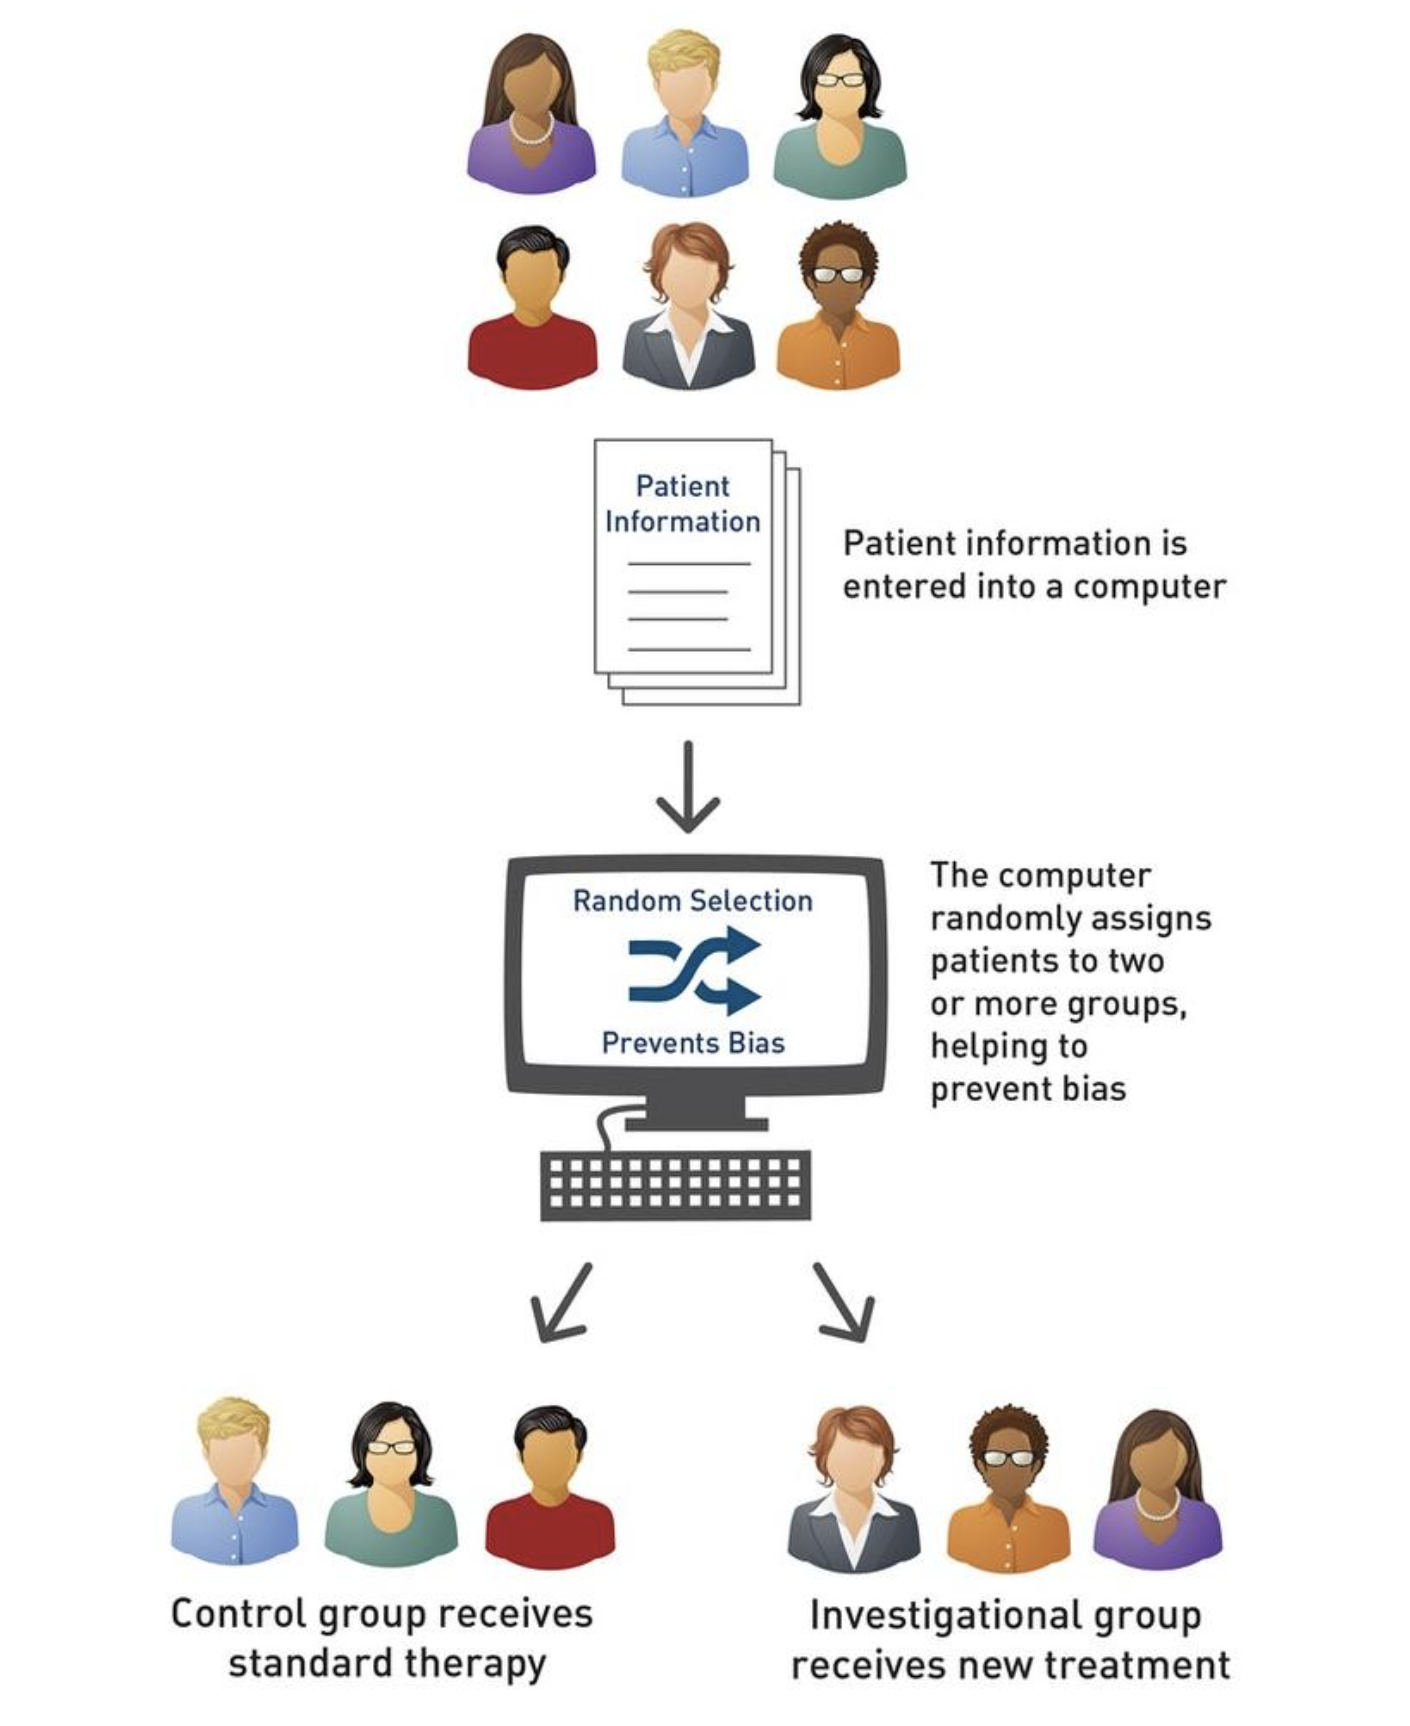
\includegraphics{parallel.png}
\href{https://www.cancer.gov/about-cancer/treatment/clinical-trials/what-are-trials/randomization/clinical-trial-randomization-infographic}{그림 출처}

임상실험에서 요인은 치료 방법(treatmanet)이며 보통의 경우 2개의 수준를 가진다. 두 개의 수준 중 하나는 실험자가 연구대상으로 고려한 효과가 기대되는 치료/약품(active)이며 다른 하나의 수준은 제어 수준(control)이다. 임상실험에서는 대부분의 경우 효과가 있는 치료나 약품을 적용하지 않아도 \textbf{위약효과(placebo effect)}가 나타나기 때문에 실험자가 사용하려고 하는 치료법의 효과는 언제나 제어군에서 나타난 효과와의 차이로 파악해야 한다.

병렬 계획은 환자가 임의로 선택된 하나의 치료/약품만 받는 실험을 말한다. 참고로 뒤에서 살펴보겠지만 환자가 2개 이상의 치료을 받는 교차실험(crossover design)도 있다.

\hypertarget{uxacf5uxbd84uxc0b0-uxbd84uxc11duxc758-uxac1cuxc694}{%
\section{공분산 분석의 개요}\label{uxacf5uxbd84uxc0b0-uxbd84uxc11duxc758-uxac1cuxc694}}

많은 임상 실험에서는 실험의 질과 수준이 실제 환자를 치료하는 환경과 동일하게 유지하는 것을 원칙으로 한다. 따라서 임상실험은 동장이나 연구실에서 수행하는 매우 정교하게 통제된 실험과 다르게 치료방법 외의 다양한 요인들이 영향을 미치게 된다. 이러한 다양한 요인들은 맹검화(blinding) 등 다양한 실험 기법을 사용하여 통제된다.

다양한 요인의 영향을 통제하려는 시도에도 불구하고 대표적으로 실험의 결과에 영향을 미치는 요인은 환자의 초기 상태(baseline)과 기관/병원(center/hospital effect)이다. 임상실험에 참가하는 환자들은 약품을 처리받기 전의 상태가 모두 다르기 때문에 처리의 효과뿐만이 아니라 환자의 초기 상태도 최종 반응값에 영향을 미친다. 또한 대부분의 임상실험은 여러 개의 병원(또는 지역, 나라)에서 동시에 실행되므로 병원, 지역, 국가의 특성에 따라서 임상시험의 결과에 영향을 미친다.

이렇게 실험에서 주요하게 고려하는 요인인 아닌 다른 요인이 영향을 미친다고 판단될 때 그 요인을 \textbf{공변량 (covariate)} 라고 부르며 공변량을 모형에 포함시키는 분석을 \textbf{공분산분석(Analysis of Covariance; ANOCOVA)}라고 부른다.

공변량의 형태는 보통 실험 단위가 가지고 있는 특성이나 실험자가 가진 특성을 반영한다. 예를 들어 다음과 같은 공변량의 형태가 있다.

\begin{itemize}
\tightlist
\item
  교육 방법을 비교하는 실험에서 학생들이 가진 학습 역량
\item
  혈압 강하를 위한 약품에 대한 실험에서 임상 참가 전 환자의 혈압과 나이
\item
  천식에 대한 약품 실험이 여러 국가에서 실행될때 국가의 효과
\item
  암을 진단하는 방법에 대한 임상 실험이 다수의 병원에서 진행될 때 병원의 효과
\end{itemize}

일반적으로 임상실험이나 관측연구에서는 관심이 있는 처리(treatment)나 요인(factor)뿐만 아니라 다른 요인들도 반응변수에 영향을 미친다. 이러한 다른 요인들의 영향을 제거하기 위한 방법은 여러가지가 있지만 실험인 경우 임의화 방법(randomization)으로 그 영향을 상쇄시킬 수 도 있고 관측연구인 경우에는 사례-대조연구 방법을 이용하여 그 영향을 최소화하려고 노력을 한다. 하지만 다양한 통제 방법에도 불구하고 여러 가지 변수들이 반응변수에 영향을 미친다. 이러한 경우에 중요한 요인을 모형에 포함시켜서 그 영향을 반영하고 동시에 자료의 변동을 부가적으로 설명해주는 방법이 공분산 분석이다.

\hypertarget{uxacf5uxbd84uxc0b0uxbd84uxc11duxc758-uxbaa8uxd615}{%
\section{공분산분석의 모형}\label{uxacf5uxbd84uxc0b0uxbd84uxc11duxc758-uxbaa8uxd615}}

실험에서 공변량은 연속형 변수일 수도 있고 범주형일 수 도 있다. 만약 공변량이 범주형 변수인 경우 분석의 방법은 이원배치 분산분석과 매우 유사하다. 이 절에서는 공변량은 연속형 변수라고 가정하고 분석 방법을 논의할 것이다. 또한 공변량이 2개 이상인 경우도 있지만 이 절에서는 공변량이 하나인 경우만 고려한다.

공분산분석의 모형은 일원배치 분산분석 모형(처리의 수는 \(a\)개, 반복수는 \(r\))에 공변량 \(x\)의 효과를 다음과 같이 더해주는 것이다.

\begin{equation} 
y_{ij} = \mu + \alpha_i + \beta(x_{ij} - \bar x_{..}) + e_{ij}, 
\quad i=1,2,\dots,a, ~~ j=1,2,\dots,r
\label{eq:ancovamodel1}
\end{equation}

모형 \eqref{eq:ancovamodel1}에서 \(x_{ij}\)는 관측값 \(y_{ij}\)의 공변량이며 이를 중심화(centering)하여 회귀모형의 독립변수로 표현한다. 모형 \eqref{eq:ancovamodel1} 에서 \(\bar x_{..} = sum_i sum_j x_{ij}/(ar)\) 로 공변량 값의 전체 평균이다.

참고로 공변량을 중심화 하지 않는 모형은 다음과 같이 표현할 수 있다.

\begin{align*}
y_{ij} & = \mu + \alpha_i + \beta(x_{ij} - \bar x_{..}) + e_{ij} \\
  & = \beta_0 + \alpha_i + \beta x_{ij} + e_{ij} \\
  & = \beta_{0i} + \beta x_{ij} + e_{ij}
\end{align*}

\hypertarget{uxbaa8uxc218uxc758-uxcd94uxc815uxacfc-uxac00uxc124-uxac80uxc815}{%
\section{모수의 추정과 가설 검정}\label{uxbaa8uxc218uxc758-uxcd94uxc815uxacfc-uxac00uxc124-uxac80uxc815}}

모형 \eqref{eq:ancovamodel1}에서 각 모수의 추정은 최소제곱법을 이용하여 추정하며 부가조건 \(\sum_i \alpha_i =0\) 을 이용하면 다음과 같은 추정량을 얻을 수 있다

\begin{align*}
\hat \mu & = \bar y_{..} \\
\hat \alpha_i & =\bar y_{i.} - \bar y_{..} -\hat \beta(\bar x_{i.} -\bar x_{..}) \\
\hat \beta & =  \frac{ \sum_i \sum_j (x_{ij} - \bar x_{i.})(y_{ij}-\bar y_{i.})}{\sum_i \sum_j (x_{ij} - \bar x_{i.})^2}
\end{align*}

ANCOVA 모형에서는 다음과 같은 두 가지 가설을 검정할 수 있다.

ANOVA 모형에서와 같이 각 그룹의 평균에 대한 검정을 할 수 있고

\begin{equation*}
H_0: \alpha_1 = \alpha_2 =...=\alpha_a =0  \quad \text{vesus} \quad H_1: \text{ not } H_0 
\end{equation*}

또한 공변량의 효과에 대한 검정도 할 수 있다.

\begin{equation} 
H_0: \beta =0  \quad \text{vesus} \quad H_1: \beta \ne 0 
\label{eq:hypoancova}
\end{equation}

\hypertarget{uxc608uxc81c-uxd608uxc555-uxac15uxd558uxb97c-uxc704uxd55c-uxc784uxc0c1-uxc2e4uxd5d8}{%
\section{예제: 혈압 강하를 위한 임상 실험}\label{uxc608uxc81c-uxd608uxc555-uxac15uxd558uxb97c-uxc704uxd55c-uxc784uxc0c1-uxc2e4uxd5d8}}

공분산분석의 개념을 이해앟기 위한 예제로서 혈압 강하를 위한 임상 실험에서 얻는 자료를 분석해 보자.

자료는 \citep{chen2017clinical} 에 나온 자료이며 화일 \href{}{dbp.txt} 에 저장되어 있다.

혈압 강하를 위한 임상실험은 2개의 처리 집단(\texttt{A} 와 \texttt{B}) 로 각각 20명이 실험에 참가하였다. 약을 복용하기 전에 혈압을 측정하고(\texttt{DBP1}) 약을 복용한 후 한 달 간격으로 4번 측정을 하였다 (\texttt{DBP2}-\texttt{DBP5}).

최종적으로 관심있는 반응변수는 약품을 복용하기 전 혈압에서 4개월 후 혈압이 변화한 차이이다.
따라서 반응변수 \texttt{diff} 는 \texttt{DBP5}에서 \texttt{DBP1}을 뺀 값이다.

또한 공변량으로서 성별(\texttt{Sex})과 연령(\texttt{Age})를 측정하였다. 공분산분석에서는 공변량으로 연령을 고려할 것이다.

다음은 화일에서 자료를 읽고 정리하는 프로그램이다.

\begin{Shaded}
\begin{Highlighting}[]
\NormalTok{dpb }\OtherTok{\textless{}{-}} \FunctionTok{read.csv}\NormalTok{(}\StringTok{"dbp.txt"}\NormalTok{, }\AttributeTok{sep=}\StringTok{""}\NormalTok{, }\AttributeTok{header=}\ConstantTok{TRUE}\NormalTok{)}
\NormalTok{df }\OtherTok{\textless{}{-}}\NormalTok{ dpb }\SpecialCharTok{\%\textgreater{}\%} \FunctionTok{mutate}\NormalTok{(}\AttributeTok{diff =}\NormalTok{ DBP5 }\SpecialCharTok{{-}}\NormalTok{DBP1)}
\FunctionTok{head}\NormalTok{(df)}
\end{Highlighting}
\end{Shaded}

\begin{verbatim}
##   Subject TRT DBP1 DBP2 DBP3 DBP4 DBP5 Age Sex diff
## 1       1   A  114  115  113  109  105  43   F   -9
## 2       2   A  116  113  112  103  101  51   M  -15
## 3       3   A  119  115  113  104   98  48   F  -21
## 4       4   A  115  113  112  109  101  42   F  -14
## 5       5   A  116  112  107  104  105  49   M  -11
## 6       6   A  117  112  113  104  102  47   M  -15
\end{verbatim}

이제 두 처리 그룹간에 혈압의 변화 \texttt{diff} 에 대하여 기초통계량으로 살펴보자.

\begin{Shaded}
\begin{Highlighting}[]
\NormalTok{dfs }\OtherTok{\textless{}{-}}\NormalTok{ df }\SpecialCharTok{\%\textgreater{}\%} \FunctionTok{group\_by}\NormalTok{(TRT)  }\SpecialCharTok{\%\textgreater{}\%}  \FunctionTok{summarise}\NormalTok{(}\AttributeTok{mean=}\FunctionTok{mean}\NormalTok{(diff), }\AttributeTok{median=} \FunctionTok{median}\NormalTok{(diff), }\AttributeTok{sd=}\FunctionTok{sd}\NormalTok{(diff), }\AttributeTok{min=}\FunctionTok{min}\NormalTok{(diff), }\AttributeTok{max=}\FunctionTok{max}\NormalTok{(diff))}
\NormalTok{dfs}
\end{Highlighting}
\end{Shaded}

\begin{verbatim}
## # A tibble: 2 x 6
##   TRT    mean median    sd   min   max
##   <chr> <dbl>  <dbl> <dbl> <int> <int>
## 1 A     -15.2  -15    2.97   -21    -9
## 2 B      -4.8   -5.5  2.42    -8     1
\end{verbatim}

두 처리 그룹간에 혈압의 변화에 대하여 그림으로 살펴보자.

\begin{Shaded}
\begin{Highlighting}[]
\FunctionTok{ggplot}\NormalTok{(df, }\FunctionTok{aes}\NormalTok{(TRT, diff)) }\SpecialCharTok{+}  \FunctionTok{geom\_boxplot}\NormalTok{()}
\end{Highlighting}
\end{Shaded}

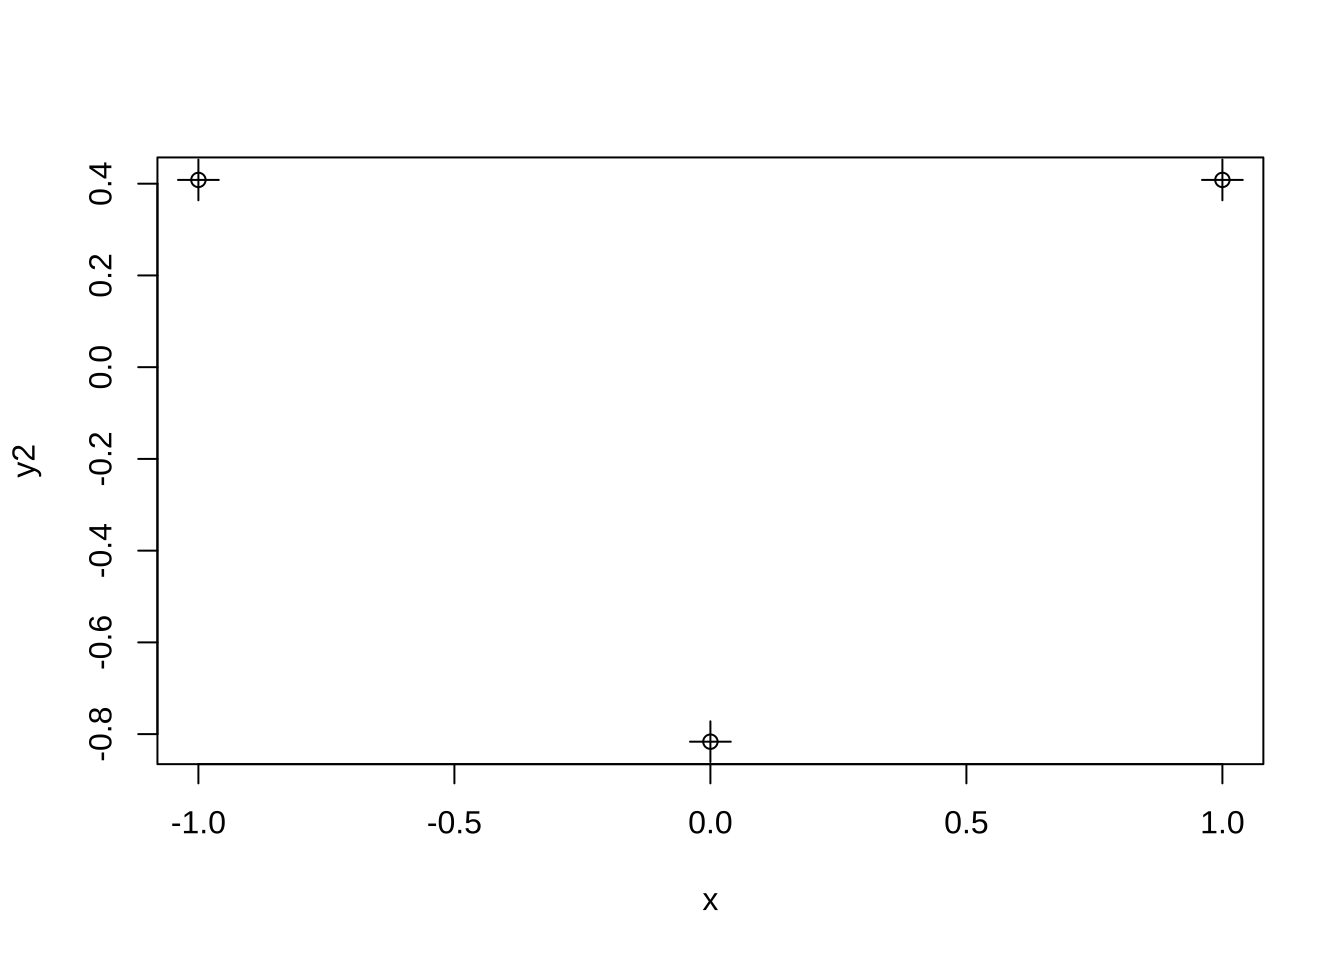
\includegraphics{Clinical-Trial_files/figure-latex/unnamed-chunk-4-1.pdf}

\texttt{A} 그룹이 \texttt{B} 그룹보다 평균적으로 혈압이 약 10 mmHg 더 감소하였다.

\hypertarget{uxbd84uxc0b0uxbd84uxc11d}{%
\section{분산분석}\label{uxbd84uxc0b0uxbd84uxc11d}}

\hypertarget{uxacf5uxbcc0uxb7c9uxc774-uxc5c6uxb294-uxc77cuxc6d0uxbc30uxce58uxbc95uxc5d0uxc11cuxc758-uxbd84uxc0b0uxbd84uxc11d}{%
\subsection{공변량이 없는 일원배치법에서의 분산분석}\label{uxacf5uxbcc0uxb7c9uxc774-uxc5c6uxb294-uxc77cuxc6d0uxbc30uxce58uxbc95uxc5d0uxc11cuxc758-uxbd84uxc0b0uxbd84uxc11d}}

우리는 아래와 같은 일원배치 실험계획에서 처리 효과에 대한 검정을 위한 분산분석표가 아래와 같이 주어지는 것을 배웠다.

\[ y_{ij} = \mu + \alpha_i + e_{ij} \]

\begin{longtable}[]{@{}crrrcr@{}}
\toprule
\begin{minipage}[b]{(\columnwidth - 5\tabcolsep) * \real{0.18}}\centering
요인\strut
\end{minipage} & \begin{minipage}[b]{(\columnwidth - 5\tabcolsep) * \real{0.08}}\raggedleft
제곱합\strut
\end{minipage} & \begin{minipage}[b]{(\columnwidth - 5\tabcolsep) * \real{0.19}}\raggedleft
자유도\strut
\end{minipage} & \begin{minipage}[b]{(\columnwidth - 5\tabcolsep) * \real{0.19}}\raggedleft
평균제곱합\strut
\end{minipage} & \begin{minipage}[b]{(\columnwidth - 5\tabcolsep) * \real{0.11}}\centering
\(F_0\)\strut
\end{minipage} & \begin{minipage}[b]{(\columnwidth - 5\tabcolsep) * \real{0.26}}\raggedleft
p-값\strut
\end{minipage}\tabularnewline
\midrule
\endhead
\begin{minipage}[t]{(\columnwidth - 5\tabcolsep) * \real{0.18}}\centering
처리\strut
\end{minipage} & \begin{minipage}[t]{(\columnwidth - 5\tabcolsep) * \real{0.08}}\raggedleft
\(SS_A\)\strut
\end{minipage} & \begin{minipage}[t]{(\columnwidth - 5\tabcolsep) * \real{0.19}}\raggedleft
\(\phi_A = a-1\)\strut
\end{minipage} & \begin{minipage}[t]{(\columnwidth - 5\tabcolsep) * \real{0.19}}\raggedleft
\(MS_A=SS_A/\phi_A\)\strut
\end{minipage} & \begin{minipage}[t]{(\columnwidth - 5\tabcolsep) * \real{0.11}}\centering
\(F_0=MS_A/MS_E\)\strut
\end{minipage} & \begin{minipage}[t]{(\columnwidth - 5\tabcolsep) * \real{0.26}}\raggedleft
\(P[F(\phi_A, \phi_E) > F_0 ]\)\strut
\end{minipage}\tabularnewline
\begin{minipage}[t]{(\columnwidth - 5\tabcolsep) * \real{0.18}}\centering
잔차\strut
\end{minipage} & \begin{minipage}[t]{(\columnwidth - 5\tabcolsep) * \real{0.08}}\raggedleft
\(SS_E\)\strut
\end{minipage} & \begin{minipage}[t]{(\columnwidth - 5\tabcolsep) * \real{0.19}}\raggedleft
\(\phi_E=a(r-1)\)\strut
\end{minipage} & \begin{minipage}[t]{(\columnwidth - 5\tabcolsep) * \real{0.19}}\raggedleft
\(MS_E=SS_E/\phi_E\)\strut
\end{minipage} & \begin{minipage}[t]{(\columnwidth - 5\tabcolsep) * \real{0.11}}\centering
\strut
\end{minipage} & \begin{minipage}[t]{(\columnwidth - 5\tabcolsep) * \real{0.26}}\raggedleft
\strut
\end{minipage}\tabularnewline
\begin{minipage}[t]{(\columnwidth - 5\tabcolsep) * \real{0.18}}\centering
총합\strut
\end{minipage} & \begin{minipage}[t]{(\columnwidth - 5\tabcolsep) * \real{0.08}}\raggedleft
\(SS_T\)\strut
\end{minipage} & \begin{minipage}[t]{(\columnwidth - 5\tabcolsep) * \real{0.19}}\raggedleft
\(\phi_T = ar-1\)\strut
\end{minipage} & \begin{minipage}[t]{(\columnwidth - 5\tabcolsep) * \real{0.19}}\raggedleft
\strut
\end{minipage} & \begin{minipage}[t]{(\columnwidth - 5\tabcolsep) * \real{0.11}}\centering
\strut
\end{minipage} & \begin{minipage}[t]{(\columnwidth - 5\tabcolsep) * \real{0.26}}\raggedleft
\strut
\end{minipage}\tabularnewline
\bottomrule
\end{longtable}

위의 분산분석표에서 다음과 같이 제곱합의 분해가 얻어진다.

\begin{equation}
SS_T = SS_A + SS_E
\label{eq:ssdecomp1}
\end{equation}

혈압 자료에 처리 효과만 있는 일원배치법으로 분산분석표를 구해보자. 두 처리 집단 사이에 혈압의 변화에 대한 차이는 매우 유의하다. 참고로 가설 검정에 이용되는 F-값은 147.63 이다.

\begin{Shaded}
\begin{Highlighting}[]
\NormalTok{lmres1 }\OtherTok{\textless{}{-}} \FunctionTok{lm}\NormalTok{(diff}\SpecialCharTok{\textasciitilde{}}\NormalTok{TRT, }\AttributeTok{data=}\NormalTok{df)}
\NormalTok{lmaov1 }\OtherTok{\textless{}{-}} \FunctionTok{anova}\NormalTok{(lmres1)}
\NormalTok{lmaov1}
\end{Highlighting}
\end{Shaded}

\begin{verbatim}
## Analysis of Variance Table
## 
## Response: diff
##           Df Sum Sq Mean Sq F value    Pr(>F)    
## TRT        1 1081.6 1081.60  147.63 1.169e-14 ***
## Residuals 38  278.4    7.33                      
## ---
## Signif. codes:  0 '***' 0.001 '**' 0.01 '*' 0.05 '.' 0.1 ' ' 1
\end{verbatim}

\hypertarget{uxacf5uxbcc0uxb7c9uxc774-uxc788uxb294-uxc77cuxc6d0uxbc30uxce58uxbc95uxc5d0uxc11cuxc758-uxbd84uxc0b0uxbd84uxc11d}{%
\subsection{공변량이 있는 일원배치법에서의 분산분석}\label{uxacf5uxbcc0uxb7c9uxc774-uxc788uxb294-uxc77cuxc6d0uxbc30uxce58uxbc95uxc5d0uxc11cuxc758-uxbd84uxc0b0uxbd84uxc11d}}

공변량이 포함된 모형 \eqref{eq:ancovamodel1} 에 대한 분산분석표는 다음과 같이 주어진다.

\begin{longtable}[]{@{}crrrcr@{}}
\toprule
\begin{minipage}[b]{(\columnwidth - 5\tabcolsep) * \real{0.18}}\centering
요인\strut
\end{minipage} & \begin{minipage}[b]{(\columnwidth - 5\tabcolsep) * \real{0.08}}\raggedleft
제곱합\strut
\end{minipage} & \begin{minipage}[b]{(\columnwidth - 5\tabcolsep) * \real{0.19}}\raggedleft
자유도\strut
\end{minipage} & \begin{minipage}[b]{(\columnwidth - 5\tabcolsep) * \real{0.19}}\raggedleft
평균제곱합\strut
\end{minipage} & \begin{minipage}[b]{(\columnwidth - 5\tabcolsep) * \real{0.11}}\centering
\(F_0\)\strut
\end{minipage} & \begin{minipage}[b]{(\columnwidth - 5\tabcolsep) * \real{0.26}}\raggedleft
p-값\strut
\end{minipage}\tabularnewline
\midrule
\endhead
\begin{minipage}[t]{(\columnwidth - 5\tabcolsep) * \real{0.18}}\centering
변량\strut
\end{minipage} & \begin{minipage}[t]{(\columnwidth - 5\tabcolsep) * \real{0.08}}\raggedleft
\(SS_X\)\strut
\end{minipage} & \begin{minipage}[t]{(\columnwidth - 5\tabcolsep) * \real{0.19}}\raggedleft
\(\phi_X=1\)\strut
\end{minipage} & \begin{minipage}[t]{(\columnwidth - 5\tabcolsep) * \real{0.19}}\raggedleft
\(MS_X=SS_X/\phi_X\)\strut
\end{minipage} & \begin{minipage}[t]{(\columnwidth - 5\tabcolsep) * \real{0.11}}\centering
\(F_X=MS_X/MS_E\)\strut
\end{minipage} & \begin{minipage}[t]{(\columnwidth - 5\tabcolsep) * \real{0.26}}\raggedleft
\strut
\end{minipage}\tabularnewline
\begin{minipage}[t]{(\columnwidth - 5\tabcolsep) * \real{0.18}}\centering
처리\strut
\end{minipage} & \begin{minipage}[t]{(\columnwidth - 5\tabcolsep) * \real{0.08}}\raggedleft
\(SS_A\)\strut
\end{minipage} & \begin{minipage}[t]{(\columnwidth - 5\tabcolsep) * \real{0.19}}\raggedleft
\(\phi_A = a-1\)\strut
\end{minipage} & \begin{minipage}[t]{(\columnwidth - 5\tabcolsep) * \real{0.19}}\raggedleft
\(MS_A=SS_A/\phi_A\)\strut
\end{minipage} & \begin{minipage}[t]{(\columnwidth - 5\tabcolsep) * \real{0.11}}\centering
\(F_0=MS_A/MS_E\)\strut
\end{minipage} & \begin{minipage}[t]{(\columnwidth - 5\tabcolsep) * \real{0.26}}\raggedleft
\(P[F(\phi_A, \phi_E) > F_0 ]\)\strut
\end{minipage}\tabularnewline
\begin{minipage}[t]{(\columnwidth - 5\tabcolsep) * \real{0.18}}\centering
잔차\strut
\end{minipage} & \begin{minipage}[t]{(\columnwidth - 5\tabcolsep) * \real{0.08}}\raggedleft
\(SS'_E\)\strut
\end{minipage} & \begin{minipage}[t]{(\columnwidth - 5\tabcolsep) * \real{0.19}}\raggedleft
\(\phi_E=a(r-1)-1\)\strut
\end{minipage} & \begin{minipage}[t]{(\columnwidth - 5\tabcolsep) * \real{0.19}}\raggedleft
\(MS'_E=SS'_E/\phi_E\)\strut
\end{minipage} & \begin{minipage}[t]{(\columnwidth - 5\tabcolsep) * \real{0.11}}\centering
\strut
\end{minipage} & \begin{minipage}[t]{(\columnwidth - 5\tabcolsep) * \real{0.26}}\raggedleft
\strut
\end{minipage}\tabularnewline
\begin{minipage}[t]{(\columnwidth - 5\tabcolsep) * \real{0.18}}\centering
총합\strut
\end{minipage} & \begin{minipage}[t]{(\columnwidth - 5\tabcolsep) * \real{0.08}}\raggedleft
\(SS_T\)\strut
\end{minipage} & \begin{minipage}[t]{(\columnwidth - 5\tabcolsep) * \real{0.19}}\raggedleft
\(\phi_T = ar-1\)\strut
\end{minipage} & \begin{minipage}[t]{(\columnwidth - 5\tabcolsep) * \real{0.19}}\raggedleft
\strut
\end{minipage} & \begin{minipage}[t]{(\columnwidth - 5\tabcolsep) * \real{0.11}}\centering
\strut
\end{minipage} & \begin{minipage}[t]{(\columnwidth - 5\tabcolsep) * \real{0.26}}\raggedleft
\strut
\end{minipage}\tabularnewline
\bottomrule
\end{longtable}

이제 혈압 자료에 연령을 공변량으로 포함한 일원배치법으로 공분산분석표를 구해보자. 두 처리 집단 사이에 혈압의 변화에 대한 차이는 매우 유의하다. 참고로 가설 검정에 이용되는 F-값은 176.03 로서 공변량이 없는 경우(147.63)보다 크다.

\begin{Shaded}
\begin{Highlighting}[]
\NormalTok{lmres2 }\OtherTok{\textless{}{-}} \FunctionTok{lm}\NormalTok{(diff}\SpecialCharTok{\textasciitilde{}}\NormalTok{TRT }\SpecialCharTok{+}\NormalTok{ Age, }\AttributeTok{data=}\NormalTok{df)}
\NormalTok{lmaov2 }\OtherTok{\textless{}{-}} \FunctionTok{anova}\NormalTok{(lmres2)}
\NormalTok{lmaov2}
\end{Highlighting}
\end{Shaded}

\begin{verbatim}
## Analysis of Variance Table
## 
## Response: diff
##           Df  Sum Sq Mean Sq  F value    Pr(>F)    
## TRT        1 1081.60 1081.60 176.0395 1.228e-15 ***
## Age        1   51.07   51.07   8.3119  0.006525 ** 
## Residuals 37  227.33    6.14                       
## ---
## Signif. codes:  0 '***' 0.001 '**' 0.01 '*' 0.05 '.' 0.1 ' ' 1
\end{verbatim}

공변량이 있는 경우 분산분석표에서 다음과 같이 제곱합의 분해가 얻어진다.

\begin{equation}
SS_T = SS_A + SS_X + SS'_E
\label{eq:ssdecomp2}
\end{equation}

이제 공변량이 없는 경우의 제곱합의 분해 \eqref{eq:ssdecomp1} 과 있는 경우의 분해 \eqref{eq:ssdecomp1} 을 보면 공변량이 없는 경우의 오차제곱합이 두 개의 제곱합으로 분해되는 것을 알 수 있다.

\begin{equation}
SS_E = SS_X + SS'_E
\label{eq:anocvadecomp}
\end{equation}

즉, 만약 반응변수와 공변량의 상관관계가 크면 공변량에 대한 제곱합 \(SS_X\)가 커질 것이며 이는
공변량이 있는 모형에서 처리 효과를 검정하는 경우 사용되는 오차제곱합 \(SS'_E\) 가 공변량이 없는
경우의 \(SS_E\) 보다 작아지는 것을 알 수 있다.

결론적으로 반응변수와 공변량의 상관관계가 크면, 공변량을 포함하는 모형에서 처리 효과를 검정하는 \(F\)-값이 공변량을 포함하지 않는 것보다 일반적으로 커지게 된다. 이는 공변량이 처리효과로 설명하지 못하는 변동 중의 일부를 설명하기 때문에 처리효과에 대한 검정력이 높아지게 된다.

공변량의 유무에 따른 제곱합의 분해의 차이를 그림으로 나타내면 다음과 같다.

\begin{Shaded}
\begin{Highlighting}[]
\NormalTok{ssq1 }\OtherTok{\textless{}{-}} \FunctionTok{data.frame}\NormalTok{(}\AttributeTok{effect=}\FunctionTok{c}\NormalTok{(}\StringTok{"TRT"}\NormalTok{, }\StringTok{"Residuals"}\NormalTok{), }\AttributeTok{sumsquare=}\NormalTok{lmaov1}\SpecialCharTok{$}\StringTok{"Sum Sq"}\NormalTok{)}
\NormalTok{ssq2 }\OtherTok{\textless{}{-}} \FunctionTok{data.frame}\NormalTok{(}\AttributeTok{effect=}\FunctionTok{c}\NormalTok{(}\StringTok{"TRT"}\NormalTok{,}\StringTok{"Age"}\NormalTok{, }\StringTok{"Residuals"}\NormalTok{), }\AttributeTok{sumsquare=}\NormalTok{lmaov2}\SpecialCharTok{$}\StringTok{"Sum Sq"}\NormalTok{)}

\FunctionTok{par}\NormalTok{(}\AttributeTok{mar =} \FunctionTok{c}\NormalTok{(}\DecValTok{2}\NormalTok{, }\DecValTok{2}\NormalTok{, }\DecValTok{2}\NormalTok{, }\DecValTok{2}\NormalTok{))}
\FunctionTok{pie}\NormalTok{(ssq1}\SpecialCharTok{$}\NormalTok{sumsquare, }\AttributeTok{labels =}\NormalTok{ ssq1}\SpecialCharTok{$}\NormalTok{effect, }\AttributeTok{main=}\StringTok{"ANOVA"}\NormalTok{)}
\FunctionTok{pie}\NormalTok{(ssq2}\SpecialCharTok{$}\NormalTok{sumsquare, }\AttributeTok{labels =}\NormalTok{ ssq2}\SpecialCharTok{$}\NormalTok{effect, }\AttributeTok{main =} \StringTok{"ANCOVA"}\NormalTok{)}
\end{Highlighting}
\end{Shaded}

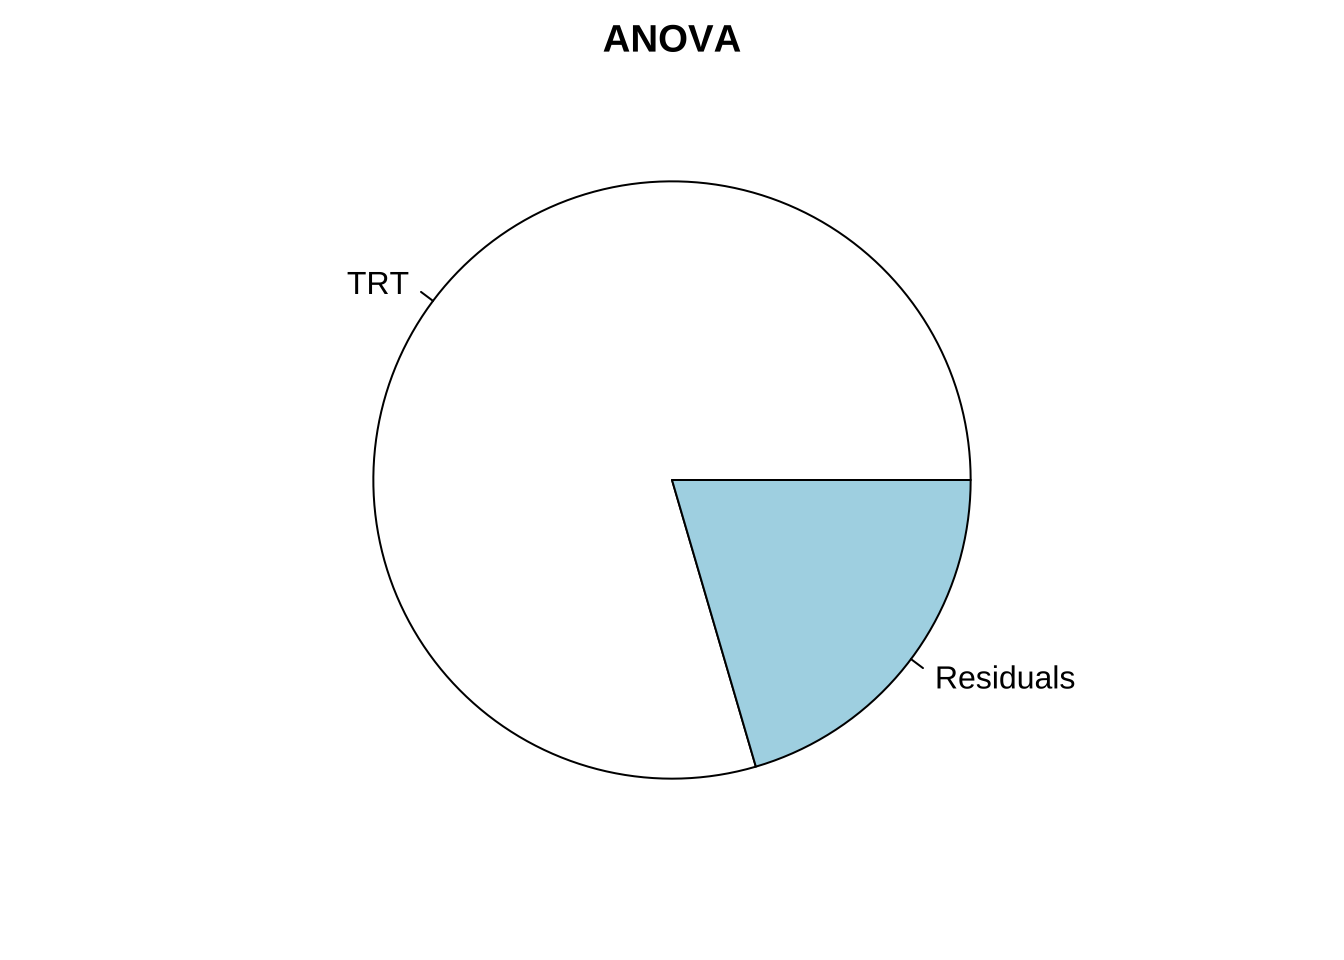
\includegraphics[width=0.5\linewidth]{Clinical-Trial_files/figure-latex/figures-side-1} 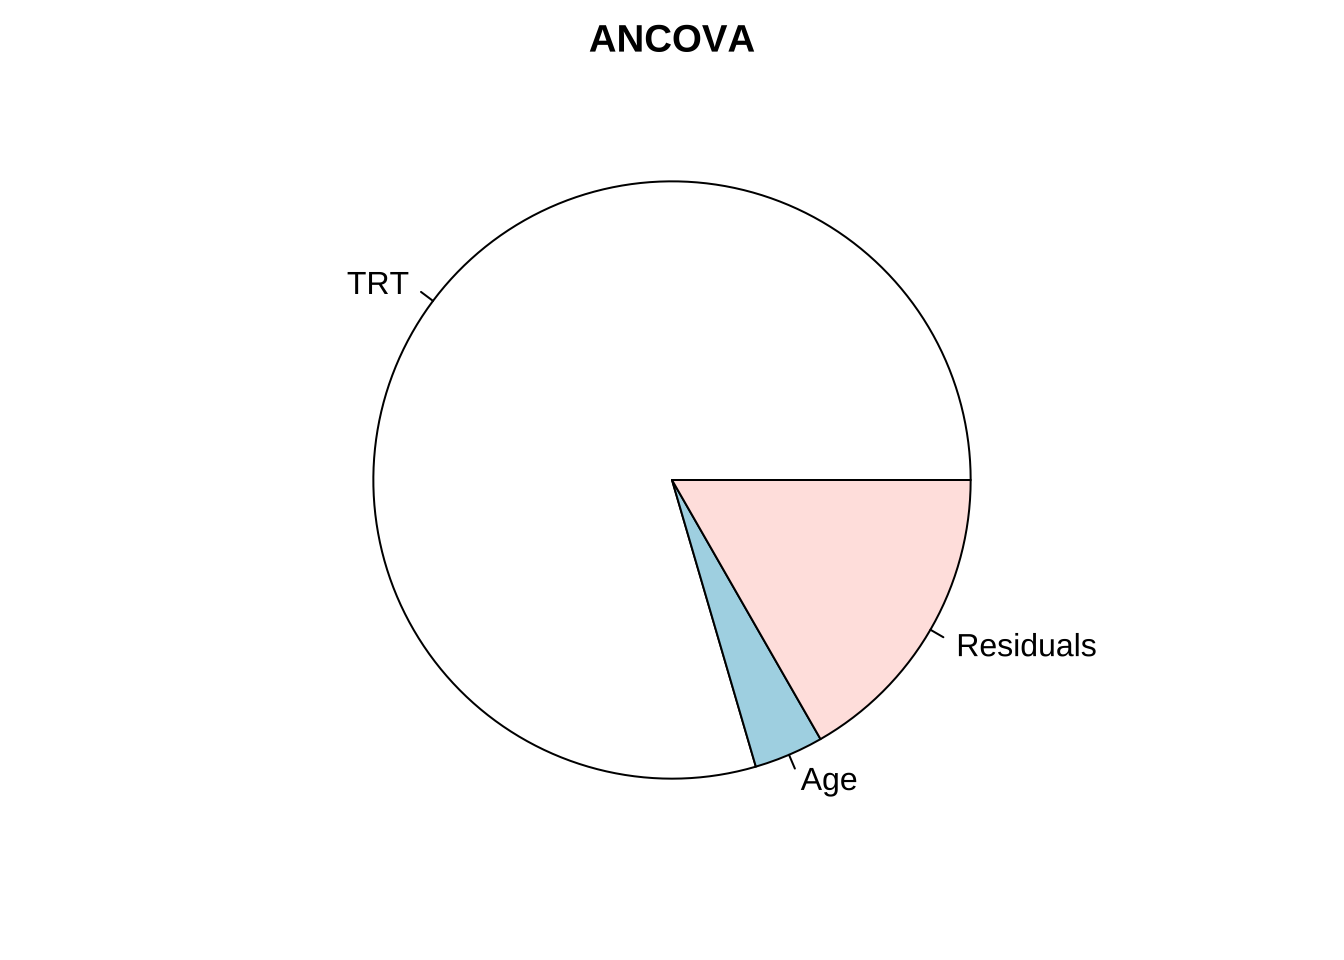
\includegraphics[width=0.5\linewidth]{Clinical-Trial_files/figure-latex/figures-side-2}

참고로 공변량을 포함하는 모형에서 오차제곱합의 자유도는 포함하지 않는 모형보다 1개가 줄어든다.
이는 공변량에 의한 제곱합의 자유도 1개가 추가되기 때문이다.

\hypertarget{uxacf5uxbd84uxc0b0uxbd84uxc11d-uxbaa8uxd615uxc758-uxd574uxc11d}{%
\section{공분산분석 모형의 해석}\label{uxacf5uxbd84uxc0b0uxbd84uxc11d-uxbaa8uxd615uxc758-uxd574uxc11d}}

이제 위에서 구한 공분산분석 모형 \eqref{eq:ancovamodel1}에 대한 추정식을 살펴보자.

\begin{Shaded}
\begin{Highlighting}[]
\FunctionTok{summary}\NormalTok{(lmres2)}
\end{Highlighting}
\end{Shaded}

\begin{verbatim}
## 
## Call:
## lm(formula = diff ~ TRT + Age, data = df)
## 
## Residuals:
##     Min      1Q  Median      3Q     Max 
## -5.9039 -1.6516 -0.0091  1.1557  5.2299 
## 
## Coefficients:
##             Estimate Std. Error t value Pr(>|t|)    
## (Intercept) -6.78086    2.97236  -2.281  0.02838 *  
## TRTB        10.13149    0.78936  12.835 3.38e-15 ***
## Age         -0.17323    0.06009  -2.883  0.00653 ** 
## ---
## Signif. codes:  0 '***' 0.001 '**' 0.01 '*' 0.05 '.' 0.1 ' ' 1
## 
## Residual standard error: 2.479 on 37 degrees of freedom
## Multiple R-squared:  0.8328, Adjusted R-squared:  0.8238 
## F-statistic: 92.18 on 2 and 37 DF,  p-value: 4.243e-15
\end{verbatim}

위의 추정 결과를 이용하여 혈압 변화의 평균에 대하여 다음과 같은 추정식을 고려할 수 있다.

\begin{Shaded}
\begin{Highlighting}[]
\FunctionTok{extract\_eq}\NormalTok{(lmres2, }\AttributeTok{use\_coefs =} \ConstantTok{TRUE}\NormalTok{) }
\end{Highlighting}
\end{Shaded}

\[
\operatorname{\widehat{diff}} = -6.78 + 10.13(\operatorname{TRT}_{\operatorname{B}}) - 0.17(\operatorname{Age})
\]

이제 처리 그룹(\texttt{A}, \texttt{B})과 연령 간의 관계를 그림으로 그려보면 다음과 같이 나타낼 수 있다.
연령이 증가하면 혈압의 강화 효과가 점점 더 커지는 것을 알 수 있으며 통계적으로도 유의하다.

\begin{Shaded}
\begin{Highlighting}[]
\FunctionTok{plot}\NormalTok{(diff}\SpecialCharTok{\textasciitilde{}}\NormalTok{Age,}\AttributeTok{las=}\DecValTok{1}\NormalTok{,}\AttributeTok{pch=}\FunctionTok{as.character}\NormalTok{(TRT), df, }\AttributeTok{xlab=}\StringTok{"Age"}\NormalTok{, }\AttributeTok{ylab=}\StringTok{"DBP Change"}\NormalTok{)}
\FunctionTok{abline}\NormalTok{(lmres2}\SpecialCharTok{$}\NormalTok{coef[}\DecValTok{1}\NormalTok{], lmres2}\SpecialCharTok{$}\NormalTok{coef[}\DecValTok{3}\NormalTok{],}\AttributeTok{lwd=}\DecValTok{2}\NormalTok{, }\AttributeTok{lty=}\DecValTok{1}\NormalTok{)}
\FunctionTok{abline}\NormalTok{(lmres2}\SpecialCharTok{$}\NormalTok{coef[}\DecValTok{1}\NormalTok{]}\SpecialCharTok{+}\NormalTok{lmres2}\SpecialCharTok{$}\NormalTok{coef[}\DecValTok{2}\NormalTok{], lmres2}\SpecialCharTok{$}\NormalTok{coef[}\DecValTok{3}\NormalTok{],}\AttributeTok{lwd=}\DecValTok{2}\NormalTok{, }\AttributeTok{lty=}\DecValTok{4}\NormalTok{)}
\end{Highlighting}
\end{Shaded}

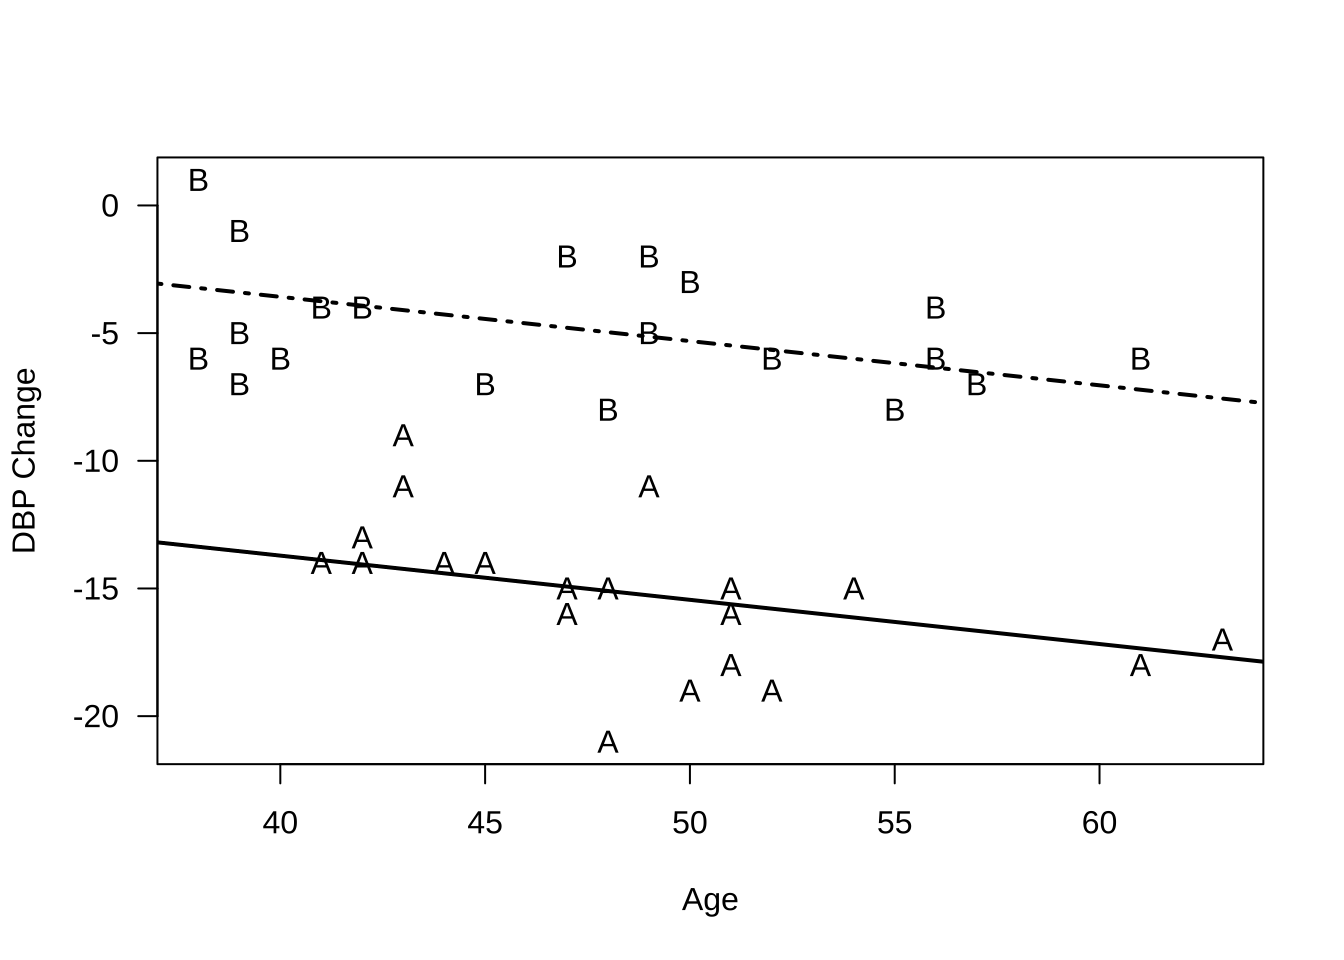
\includegraphics{Clinical-Trial_files/figure-latex/unnamed-chunk-9-1.pdf}

\hypertarget{designtype}{%
\chapter{우월성, 동등성, 비열등성}\label{designtype}}

\hypertarget{uxc784uxc0c1uxc2e4uxd5d8uxc758-uxbaa9uxc801-uxc6b0uxc6d4uxc131-uxb3d9uxb4f1uxc131-uxbe44uxc5f4uxb4f1uxc131}{%
\section{임상실험의 목적: 우월성, 동등성, 비열등성}\label{uxc784uxc0c1uxc2e4uxd5d8uxc758-uxbaa9uxc801-uxc6b0uxc6d4uxc131-uxb3d9uxb4f1uxc131-uxbe44uxc5f4uxb4f1uxc131}}

\begin{itemize}
\tightlist
\item
  우월성 (superiority)

  \begin{itemize}
  \tightlist
  \item
    T is superior to S
  \item
    Treatment T has more therapeutic effect than S.
  \end{itemize}
\item
  동등성(equivalence)

  \begin{itemize}
  \tightlist
  \item
    T is equivalent to S
  \item
    Two treatments T and S have equal therapeutic effect.
  \end{itemize}
\item
  비열등성(noninferiority)

  \begin{itemize}
  \tightlist
  \item
    T is noninferior to S
  \item
    Treatment T is not inferior to S (T is as effective as S)
  \end{itemize}
\end{itemize}

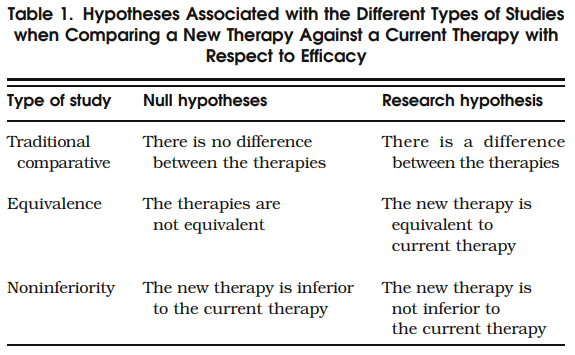
\includegraphics{equiv-meaning.png}

출처: \citet{walker2011understanding}

\hypertarget{uxd1b5uxacc4uxc801-uxac00uxc124}{%
\section{통계적 가설}\label{uxd1b5uxacc4uxc801-uxac00uxc124}}

평균이 큰 것이 좋다고 가정하자.

\begin{itemize}
\tightlist
\item
  우월성 연구의 가설
\end{itemize}

\[ H_0 : \mu_T = \mu_S  \quad \text{ vs. } \quad H_1: \mu_T \ne \mu_S   \]

\begin{itemize}
\item
  사실상 우월성 실험의 대립 가설은 \(H_1: \mu_T > \mu_S\) 이다.
\item
  우월성에 대한 가설을 아래와 같이 세울수도 있지만 거의 사용하지 않는다.
\end{itemize}

\[ H_0 : \mu_T \le  \mu_S + \delta  \quad \text{ vs. } \quad H_1: \mu_T > \mu_S +   \delta \]

\begin{itemize}
\item
  \(\delta\)는 margin 이라고 부르며 의학적(임상적)으로 우월한 차이를 보이는 치료 효과의 차이를 말한다.
\item
  동등성(equivalence)
\end{itemize}

\[ H_0 : | \mu_T - \mu_S | \ge \delta \quad \text{ vs. } \quad H_1: | \mu_T - \mu_S| < \delta \]

\begin{itemize}
\tightlist
\item
  비열등성(noninferiority)
\end{itemize}

\[ H_0  : \mu_T \le  \mu_S - \delta  \quad \text{ vs. } \quad H_1: \mu_T > \mu_S -   \delta \]

\hypertarget{uxd1b5uxacc4uxc801-uxac80uxc815-uxc808uxcc28---uxc6b0uxc6d4uxc131}{%
\section{통계적 검정 절차 - 우월성}\label{uxd1b5uxacc4uxc801-uxac80uxc815-uxc808uxcc28---uxc6b0uxc6d4uxc131}}

\begin{itemize}
\tightlist
\item
  우월성 연구의 가설
\end{itemize}

\[ H_0 : \mu_T = \mu_S  \quad \text{ vs. } \quad H_1: \mu_T \ne \mu_S   \]

\begin{itemize}
\item
  일반적인 t-검정 또는 z-검정을 사용
\item
  귀무가설의 기각 조건
\end{itemize}

\[   \frac{\hat \mu_T - \hat \mu_S}{se(\hat \mu_T - \hat \mu_S)} > c_{\alpha/2} \]
또는

\[   (\hat \mu_T - \hat \mu_S) - c_{\alpha/2}  se(\hat \mu_T - \hat \mu_S) > 0  \]

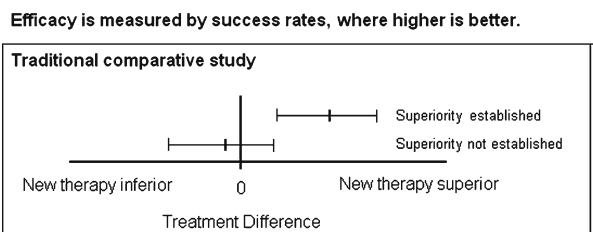
\includegraphics{equiv-super.png}

출처: \citet{walker2011understanding}

\hypertarget{uxd1b5uxacc4uxc801-uxac80uxc815-uxc808uxcc28---uxbe44uxc5f4uxb4f1uxc131}{%
\section{통계적 검정 절차 - 비열등성}\label{uxd1b5uxacc4uxc801-uxac80uxc815-uxc808uxcc28---uxbe44uxc5f4uxb4f1uxc131}}

\begin{itemize}
\tightlist
\item
  비열등성의 가설
\end{itemize}

\begin{equation}
H_0 : H_0 : \mu_T \le  \mu_S - \delta  \quad \text{ vs. } \quad H_1: \mu_T > \mu_S -   \delta
\label{eq:noninf}
\end{equation}

\begin{itemize}
\item
  일반적인 t-검정 또는 z-검정을 사용
\item
  귀무가설의 기각 조건
\end{itemize}

\[   (\hat \mu_T - \hat \mu_S) - c_{\alpha} ~ se(\hat \mu_T - \hat \mu_S) > -\delta  \]

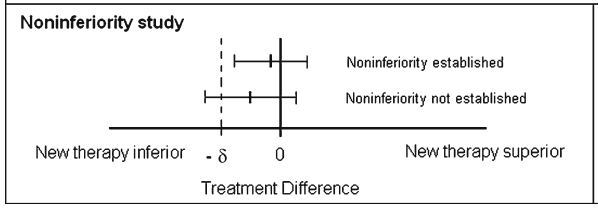
\includegraphics{equiv-inf.png}

출처: \citet{walker2011understanding}

\hypertarget{uxd1b5uxacc4uxc801-uxac80uxc815-uxc808uxcc28---uxb3d9uxb4f1uxc131}{%
\section{통계적 검정 절차 - 동등성}\label{uxd1b5uxacc4uxc801-uxac80uxc815-uxc808uxcc28---uxb3d9uxb4f1uxc131}}

-동등성 가설

\begin{equation}
H_0 : | \mu_T - \mu_S | \ge \delta \quad \text{ vs. } \quad H_1: | \mu_T - \mu_S| < \delta
\label{eq:equihypo}
\end{equation}

\begin{itemize}
\item
  일반적인 t-검정 또는 z-검정이 아닌 \textbf{the two one-sided test}를 사용
\item
  가설 \eqref{eq:equihypo}의 귀무가설은 다음 두 개의 단측 귀무 가설의 합집합니다.
\end{itemize}

\begin{equation}
H_{01} :  \mu_T - \mu_S  \ge \delta \quad  \quad H_{02} :  \mu_T - \mu_S  \le  -\delta
\label{eq:twoequihypo}
\end{equation}

따라서 식 \eqref{eq:twoequihypo}에 있는 두 개의 가설이 모두 기각되면 식 \eqref{eq:equihypo}에 있는 동등성 가설을 기각할 수 있다.

\begin{itemize}
\tightlist
\item
  \textbf{the two one-sided test}는 다음과 같은 두 조건이 만족되면 귀무가설을 기각한다.
\end{itemize}

\[  
\frac{\hat \mu_T - \hat \mu_S - \delta}{se(\hat \mu_T - \hat \mu_S)} < - c_{\alpha}
~~\text{ and }~~~ \frac{\hat \mu_T - \hat \mu_S + \delta}{se(\hat \mu_T - \hat \mu_S)} > c_{\alpha}
\]

위의 귀무가설 기각 조건은 다음과 동일하다. 즉 \(100(1-2\alpha)\)\% 신뢰구간이 \((-\delta, \delta)\) 안에 존재하면 귀무가설을 기각한다.

\[ 
-\delta < (\hat \mu_T - \hat \mu_S) -  c_{\alpha} ~~se(\hat \mu_T - \hat \mu_S) < 
(\hat \mu_T - \hat \mu_S) + c_{\alpha}~~ se(\hat \mu_T - \hat \mu_S) < \delta
\]

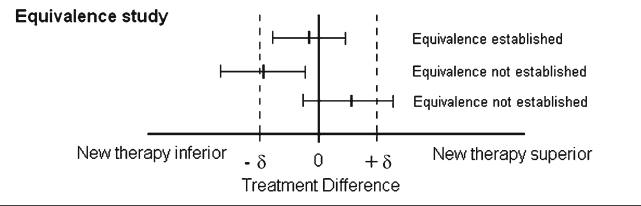
\includegraphics{equiv-equiv.png}

\hypertarget{uxb3d9uxb4f1uxc131-uxac80uxc815uxc758-size-uxc640-uxc720uxc758uxc218uxc900}{%
\section{동등성 검정의 Size 와 유의수준}\label{uxb3d9uxb4f1uxc131-uxac80uxc815uxc758-size-uxc640-uxc720uxc758uxc218uxc900}}

\begin{itemize}
\tightlist
\item
  \(100(1-2\alpha)\)\% 신뢰구간을 이용하는 경우 검정의 Size 와 유의수준은 ? ( \citet{kang2008} 참조)
\end{itemize}

\hypertarget{cross}{%
\chapter{교차실험과 동등성 검정}\label{cross}}

\hypertarget{uxc0dduxccb4uxc774uxc6a9uxb960bioavailability}{%
\section{생체이용률(Bioavailability)}\label{uxc0dduxccb4uxc774uxc6a9uxb960bioavailability}}

\begin{itemize}
\item
  the rate and extent to which the active ingredient is absorbed from a drug product and becomes available at the site of action
\item
  주성분 또는 그 활성대사체가 제제로부터 전신순환혈로 흡수되는 속도와 양의 비율
\item
  Pharmacokinetic (PK) measures (평가항목) of bioavailability

  \begin{itemize}
  \tightlist
  \item
    \(AUC_t\): Area under the blood or plasma concentration-time curve; 일정시간까지 혈중농도-시간곡선하면적
  \item
    \(C_{max}\): Maximum Concentration; 최고혈중농도
  \item
    \(T_{max}\): Time to Maximum Concentration; 최고혈중농도 도달시간
  \end{itemize}
\end{itemize}

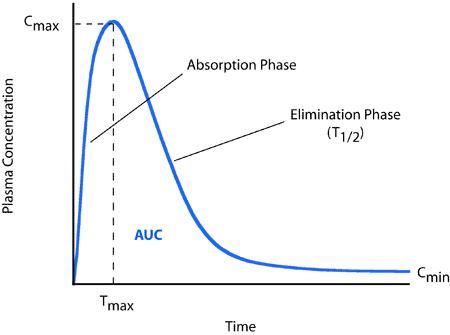
\includegraphics{plasma.jpg}

\hypertarget{uxc57duxd488-uxc8fcuxc131uxbd84uxc758-uxc0dduxccb4uxc774uxc6a9uxb960uxc758-uxd3c9uxade0uxc801-uxbcc0uxd654}{%
\section{약품 주성분의 생체이용률의 평균적 변화}\label{uxc57duxd488-uxc8fcuxc131uxbd84uxc758-uxc0dduxccb4uxc774uxc6a9uxb960uxc758-uxd3c9uxade0uxc801-uxbcc0uxd654}}

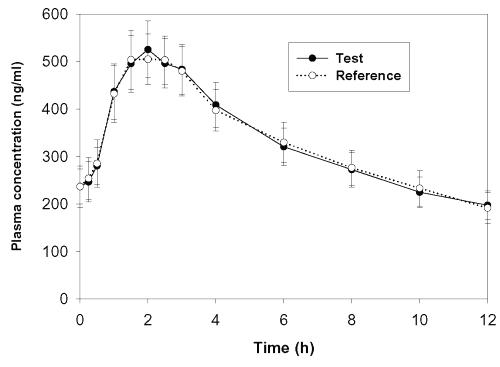
\includegraphics{bioequi.jpg}

\hypertarget{uxc0dduxbb3cuxd559uxc801uxb3d9uxb4f1uxc131uxc758-uxc815uxc758-fda-uxacfc-kfda}{%
\section{생물학적동등성의 정의: FDA 과 KFDA}\label{uxc0dduxbb3cuxd559uxc801uxb3d9uxb4f1uxc131uxc758-uxc815uxc758-fda-uxacfc-kfda}}

\begin{itemize}
\item
  Bioequivalence by FDA

  absence of a significant difference in Bioavailability between two formulations\ldots. when administered at the same molar dose under similar conditions in an appropriately designed study

  \begin{itemize}
  \item
    in vivo: Bioequivalence
  \item
    in vitro: Bioequivalence
  \end{itemize}
\item
  KFDA
\end{itemize}

의약품동등성시험이란 그 주성분 ·함량 및 제형이 동일한 두 제제에 대한 의약품동등성을 입증하기 위해 실시하는
생물학적동등성시험, 비교용출시험, 비교붕해등 기타시험의 생체내·외 시험을 말한다.

\hypertarget{uxc0dduxbb3cuxd559uxc801uxb3d9uxb4f1uxc131-uxc2e4uxd5d8uxc758-uxc124uxacc4}{%
\section{생물학적동등성 실험의 설계}\label{uxc0dduxbb3cuxd559uxc801uxb3d9uxb4f1uxc131-uxc2e4uxd5d8uxc758-uxc124uxacc4}}

\begin{itemize}
\item
  생체이용률(bioavailibility)은 개인간에 변동이 크다
\item
  개인효과(individual effect)를 제거하기 위한 쌍비교 t-검정 (paired t-test)의 개념을 도입
\item
  실험자가 두 개의 처리를 모두 받는다.
\item
  생동성실험은 주로 \textbf{교차시험(crossover design)}을 이용한다.
\item
  제재의 반감기가 긴 경우 등 특수한 경우는 병렬계획(Parallel design) 실험도 가능하다.
\item
  2x2 교차실험
\end{itemize}

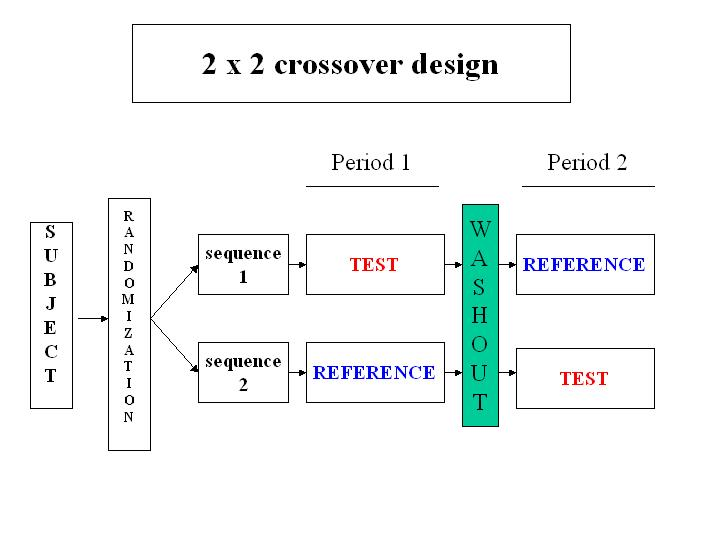
\includegraphics{design22.jpg}

\begin{itemize}
\tightlist
\item
  2x4 교차시험
\end{itemize}

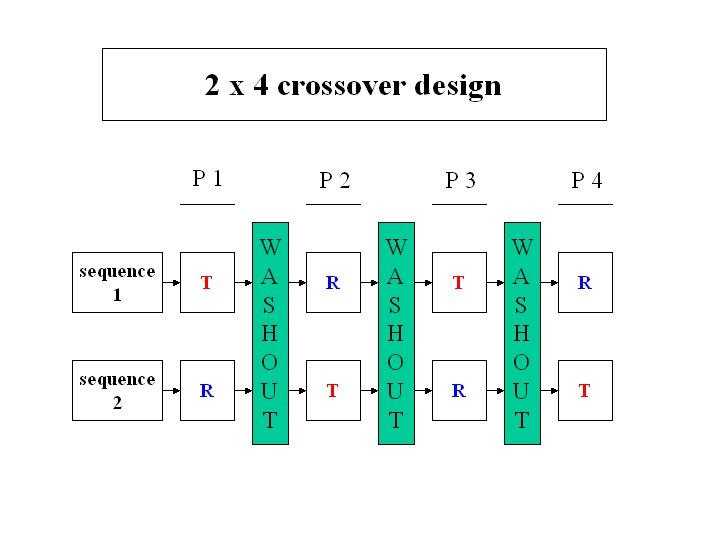
\includegraphics{design24.jpg}

\hypertarget{uxad50uxcc28uxc2e4uxd5d8uxc5d0-uxb300uxd55c-uxd1b5uxacc4uxc801-uxbaa8uxd615}{%
\section{교차실험에 대한 통계적 모형}\label{uxad50uxcc28uxc2e4uxd5d8uxc5d0-uxb300uxd55c-uxd1b5uxacc4uxc801-uxbaa8uxd615}}

\begin{itemize}
\item
  보통 10-20명의 실험 대상자
\item
  각 실험 대상자가 2개(3개 또는 4개)의 반응값(PK responses)을 가진다.
\item
  각 실험대상자의 반응값은 독립이 아니다 (correlated response; repeated measurements)
\item
  실험대상자 간의 변이가 크다 (large between-subject variation)
\item
  시험약과 대조약간의 (로그)반응값의 평균의 차이가 주 검토대상이다.
\item
  정규분포를 가정한 선형혼합모형(linear mixed model)
\end{itemize}

\hypertarget{uxd3c9uxade0uxc801-uxc0dduxbb3cuxd559uxc801uxb3d9uxb4f1uxc131uxc5d0-uxb300uxd55c-uxac00uxc124}{%
\section{평균적 생물학적동등성에 대한 가설}\label{uxd3c9uxade0uxc801-uxc0dduxbb3cuxd559uxc801uxb3d9uxb4f1uxc131uxc5d0-uxb300uxd55c-uxac00uxc124}}

\begin{itemize}
\tightlist
\item
  The absence of a significant difference (중대한 차이가 없다) in two \underline{population
  means} between two formulations .
\end{itemize}

= 시험약(T)과 대조약(R)간의 반응값의 평균의 차이: \(\mu_T-\mu_R\):

\begin{itemize}
\item
  보통 반응변수(PK response)에 로그를 취한 뒤 통계분석
\item
  \(\delta=\mu_T-\mu_R\): 시험약(T)과 대조약(R)간의 로그 반응값의 평균의 차이
\item
  평균적 생물학적동등성에 대한 가설
\end{itemize}

\[ H_0: \delta \le \delta_L ~~~or~~~ \delta \ge \delta_U   \quad vs. \quad H_1: \delta_L < \delta < \delta_U \]

\begin{itemize}
\tightlist
\item
  동등성 한계 (bioequivalence limit)
\end{itemize}

\[ \delta_L=-0.223=log(0.8) \quad and \quad \delta_U=0.223=log(1.25) \]

\begin{itemize}
\tightlist
\item
  평균적 생물학적동등성에 대한 가설(로그변환 전)
\end{itemize}

\[ H_1: 0.8 < \frac{\mu'_T}{\mu'_R} < 1.25 \]

\begin{itemize}
\tightlist
\item
  평균적 생물학적동등성을 어떤 통계적 방법으로 검정할 것인가?
\end{itemize}

\[ H_0: \delta \le \delta_L ~~~or~~~ \delta \ge \delta_U   \quad vs. \quad H_1: \delta_L < \delta < \delta_U \]

\begin{itemize}
\item
  Historical development of statistical tests for ABE

  \begin{itemize}
  \item
    Westlake (1976), Hsu (1984), Bofinger (1985, 1992), Schuirmann (1987), Liu(1990)
  \item
    Berger and Hsu (1996), Brown, Hwang, and Munk (1997), Perlman and Wu (1999), Welleck (2003), Romano (2005)
  \item
    FDA guidance: 1992, 1997, 1999, 2000 and some drafts
  \end{itemize}
\item
  가설
\end{itemize}

\[ H_0: |\mu_T-\mu_R| \ge \delta  \quad vs. \quad H_1: |\mu_T-\mu_R| < \delta \]

\begin{itemize}
\item
  신뢰구간을 이용한 방법
\item
  2개의 단측검정을 결합한 방법 (Two ones-sided tests; TOST)
\end{itemize}

\[ H_{01}: \mu_T-\mu_R  < -\delta \text{ and } H_{02}:  \mu_T-\mu_R  > \delta \]

\hypertarget{uxc2e0uxb8b0uxad6cuxac04uxc744-uxc774uxc6a9uxd55c-uxd3c9uxade0uxc801-uxc0dduxbb3cuxd559uxc801uxb3d9uxb4f1uxc131-uxac80uxc815}{%
\section{신뢰구간을 이용한 평균적 생물학적동등성 검정}\label{uxc2e0uxb8b0uxad6cuxac04uxc744-uxc774uxc6a9uxd55c-uxd3c9uxade0uxc801-uxc0dduxbb3cuxd559uxc801uxb3d9uxb4f1uxc131-uxac80uxc815}}

\begin{itemize}
\tightlist
\item
  가설
\end{itemize}

\[ H_0: |\mu_T-\mu_R| \ge \delta  \quad vs. \quad H_1: |\mu_T-\mu_R| < \delta \]

\begin{itemize}
\item
  \(\mu_T-\mu_R\) 에 대한 신뢰구간 \(C(Y)\) 를 구한다.
\item
  신뢰구간이 동등성 한계안에 포함되면 평균적 생물학적동등성 선언!
\end{itemize}

\[ C(y) \subset (-\delta,\delta) \]

\hypertarget{uxac1cuxc758-uxb2e8uxce21uxac80uxc815uxc744-uxc774uxc6a9uxd55c-uxbc29uxbc95}{%
\section{2개의 단측검정을 이용한 방법}\label{uxac1cuxc758-uxb2e8uxce21uxac80uxc815uxc744-uxc774uxc6a9uxd55c-uxbc29uxbc95}}

\begin{itemize}
\item
  정규분포 가정
\item
  각 처리에 대한 평균 \(\bar {y}_T\) 과 \(\bar {y}_R\) 는 \(\mu_T\) 과 \(\mu_R\)의 추정량
\item
  \(SE\) 를 \(\bar {y}_T-\bar {y}_R\)의 표준 오차(standard error)라고 하자
\item
  다음을 만족하면 귀무가설 \(H_0\)를 기각 (생물학적 동등성을 선언)
\end{itemize}

\[
\frac{ \bar {y}_T-  \bar {y}_R +\delta}{SE} > t_\alpha ~~\text{ and }~~
\frac{ \bar {y}_T-  \bar {y}_R -\delta}{SE} <- t_\alpha 
\]

\begin{itemize}
\tightlist
\item
  위의 귀무가설 기각조건은 아래와 동일한다 (90\% 신뢰구간이 동등성 한계안에 있다)
\end{itemize}

\[ 
[(\bar {y}_T-  \bar {y}_R - t_\alpha (SE),~ (\bar {y}_T-  \bar {y}_R + t_\alpha(SE) )] \subseteq
(-\delta,~\delta) 
\]

\begin{itemize}
\item
  TOST is a special case of intersection-union test (Berger and Hsu, 1996)
\item
  TOST is level \(2\alpha\) test, but its size is actually \(\alpha\).
\end{itemize}

\[ \text{size of test } = \sup_{H_0} P( \text{ test rejects } H_0 ) \]

\begin{itemize}
\item
  Improved tests are proposed by Berger and Hsu (1996), Brown, Hwang, and Munk (1997), Perlman and Wu (1999), Welleck (2003), Romano (2005)
\item
  But, still TOST is widely used because of its validity and simplicity
\end{itemize}

\backmatter

  \bibliography{book.bib}

\end{document}
